\documentclass[UTF8]{ctexart}
\usepackage{tikz}
\usetikzlibrary{arrows}

\tikzset{
  treenode/.style = {align=center, inner sep=0pt, text centered,
    font=\sffamily},
  arn_n/.style = {treenode, circle, white, font=\sffamily\bfseries, draw=black,
    fill=black, text width=1.5em},% arbre rouge noir, noeud noir
  arn_r/.style = {treenode, circle, red, draw=red, 
    text width=1.5em, very thick},% arbre rouge noir, noeud rouge
  arn_x/.style = {treenode, rectangle, draw=black,
    minimum width=0.5em, minimum height=0.5em}% arbre rouge noir, nil
}
\usepackage{algorithm}
\usepackage{algorithmic}
\usepackage{amsmath,amssymb}
\renewcommand{\algorithmicrequire}{ \textbf{Input:}} %Use Input in the format of Algorithm
\renewcommand{\algorithmicensure}{ \textbf{Output:}} %UseOutput in the format of Algorithm
% 参考:https://blog.csdn.net/jzwong/article/details/52399112

\begin{document}

SA22225226 李青航

\noindent \textbf{13.1-2}

插入36到图13-1中后:

如果插入的节点是红色,不再是红黑树,因为父节点35是红色,连续两个红色,破坏了红黑树规则4

如果插入的节点是黑色,不再是红黑树,因为到达36的黑高,与到达其他叶子节点的黑高不同,破坏了规则5 \\

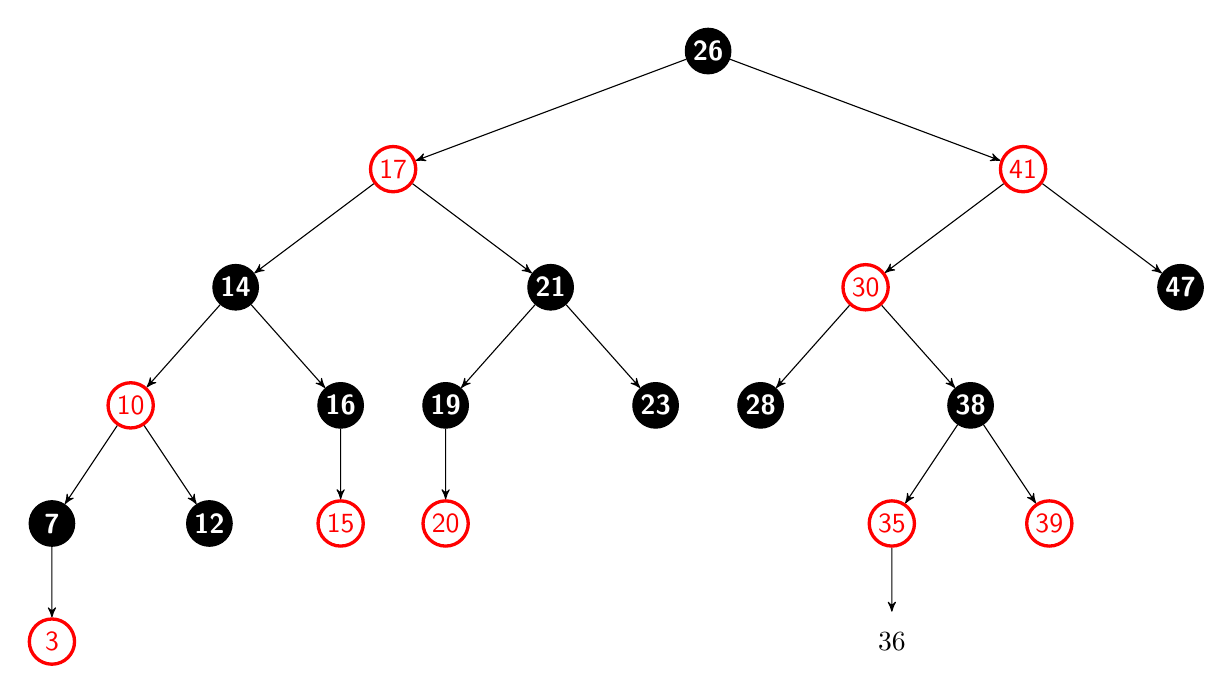
\begin{tikzpicture}[->,>=stealth',level/.style={sibling distance = 8cm/#1,
  level distance = 1.5cm}] 
\node [arn_n] {26}
    child{ node [arn_r] {17} 
            child{ node [arn_n] {14} 
            	child{ node [arn_r] {10}
            		child {node [arn_n] {7}
            			child{node [arn_r]{3}}
            		}
            		child {node [arn_n] {12}}
            	 } %for a named pointer
				child{ node [arn_n] {16}
					child{node [arn_r] {15}}
				}
            }
            child{ node [arn_n] {21}
							child{ node [arn_n] {19}
								child{node [arn_r] {20}}
							}
							child {node [arn_n]{23}}
            }                            
    }
    child{ node [arn_r] {41}
            child{ node [arn_r] {30} 
							child{ node [arn_n] {28}}
							child{ node [arn_n] {38}
								child{node [arn_r] {35}
									child{node [circle]{36}}
								}
								child{node [arn_r] {39}}
							}
            }
            child{ node [arn_n] {47}}
	}
; 
\end{tikzpicture}
~\\
\noindent \textbf{13.1-5}

一棵红黑树,根节点的黑高固定,根到所有叶节点的简单路径中,
最短的情况是“全为黑”节点,最长的情况是“红黑交替”。
所以最短与最长的情况,路径节点数相差两倍
~\\

\noindent \textbf{13.1-6}

最多的时候是每层黑红交替的满二叉树的时候,此时树高为$2k+1$,,最多节点为$2^{2k+1}-1$个

最少的时候是全黑的满二叉树,此时树高为$k+1$,最少节点为$2^{k+1}-1$个

~\\
\noindent \textbf{13.3-1}

如果插入黑的节点,就会破坏红黑树的性质5,从根到叶的简单路径的黑节点数加1,不全相同了

~\\
\noindent \textbf{13.3-2}

插入41

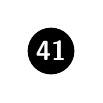
\begin{tikzpicture}[->,>=stealth',level/.style={sibling distance = 5cm/#1,
level distance = 1.5cm}] 

	\node [arn_n] {41};
  
\end{tikzpicture}

插入38

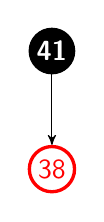
\begin{tikzpicture}[->,>=stealth',level/.style={sibling distance = 5cm/#1,
level distance = 1.5cm}] 
	
	\node [arn_n] {41}
		child{
			node [arn_r] {38}
		};
  
\end{tikzpicture}

插入31

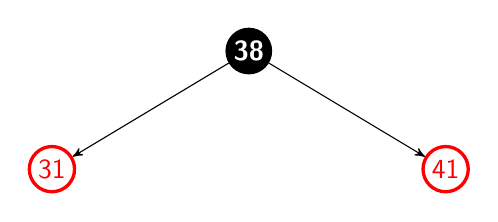
\begin{tikzpicture}[->,>=stealth',level/.style={sibling distance = 5cm/#1,
level distance = 1.5cm}] 
	
	\node [arn_n] {38}
		child{
			node [arn_r] {31}
		}
		child{
			node [arn_r] {41}
		};
  
\end{tikzpicture}

插入12

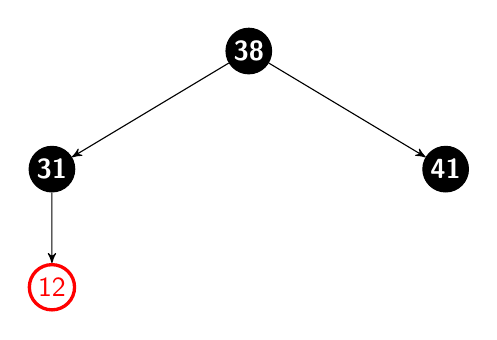
\begin{tikzpicture}[->,>=stealth',level/.style={sibling distance = 5cm/#1,
level distance = 1.5cm}] 
	
	\node [arn_n] {38}
		child{
			node [arn_n] {31}
				child{
					node [arn_r] {12}
				}
		}
		child{
			node [arn_n] {41}
		};
  
\end{tikzpicture}

插入19

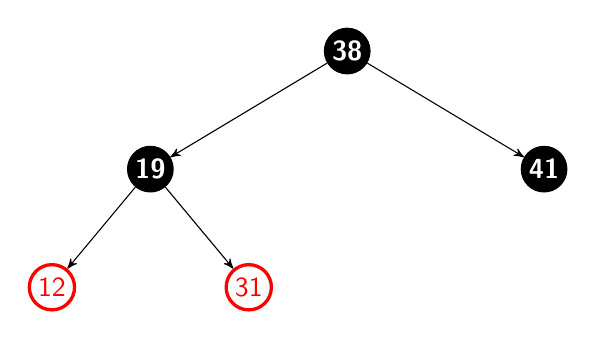
\begin{tikzpicture}[->,>=stealth',level/.style={sibling distance = 5cm/#1,
level distance = 1.5cm}] 
	
	\node [arn_n] {38}
		child{
			node [arn_n] {19}
				child{
					node [arn_r] {12}
				}
				child{
					node [arn_r] {31}
				}
		}
		child{
			node [arn_n] {41}
		};
  
\end{tikzpicture}

插入8

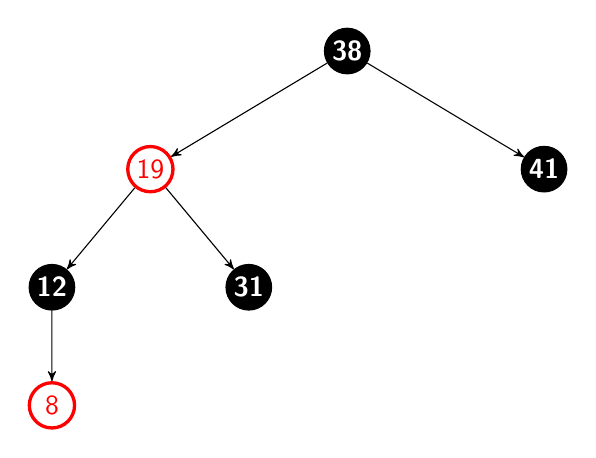
\begin{tikzpicture}[->,>=stealth',level/.style={sibling distance = 5cm/#1,
level distance = 1.5cm}] 
	
	\node [arn_n] {38}
		child{
			node [arn_r] {19}
				child{
					node [arn_n] {12}
						child{
							node [arn_r] {8}
						}
				}
				child{
					node [arn_n] {31}
				}
		}
		child{
			node [arn_n] {41}
		};
  
\end{tikzpicture}

~\\
\noindent\textbf{13.4-6}

在case 1开始,我们置$w$为结点$x$的兄弟。算法第4行判断了$w.color==red$,那就意味着$x$和$w$的父结点不能是红色的(否则违背红黑树规则4,不会父子都是红色)

\end{document}